\chapter{基于贝叶斯的无穷远参考下脑电电势的统一估计量:正则化的参考电极标准化技术}
\section{引言}
脑电参考选择是一个持续很久悬而未决的问题,导致了不一致的用法和无休止的争论。当前,平均参考(AR)和正则化点击标准化技术是两个主要,显然不能调和的竞争者。在本章中,我们提出了理论架构旨在解决参考问题,通过公式化(a) 无穷远参考下的脑电电位估计,和(b) 参考的抉择作为一个统一的贝叶斯线性逆问题,该问题可以通过最大后验估计解决。我们发现AR和REST是该统一的统计学架构非常特殊的两种情形:AR 源自于不具有生物物理学知识的先验假设;然而,REST采用了基于脑电正演模型的先验。为了同时去噪和参考估计,我们提出了AR和REST的正则化版本,分别称为rAR和rREST。二者均依赖于正则化参数,即实际的噪声信号比。传统和新的参考估计量在该统计学架构下通过仿真和真实脑电数据分析得以评价。最后,我们借助于古巴人脑计划项目中的89个被试的MRI数据和脑电数据。 仿真的具有噪声脑电作为基标准,研究表明在估计无穷远参考的脑电电位时rREST最低。同时,我们也发现真实容积传导模型改进了REST and rREST的效果。重要地是,在实际应用中,被试群体平均的传递矩阵给出了和个体传递矩阵可比的结果。最后,通过GCV的正则化参数选择接近于具有基标准的黄金参数选择。当我们分析89个被试的静息脑电,rREST 一致性地具有最低的GCV值。该章节研究通过统一的逆问题解架构提供了脑电参考问题的崭新视角。 这将可能带了更多的符合逻辑的理论公式和对于参考效果的数值评价。
\section{研究背景}
90年来,人类脑电图对于研究认知和临床神经科学来说已经成为不可或缺的工具。超高的时间分辨率、成本较低和无创性使其成为研究大脑的有力转化工具之一。然而,两个主要缺陷:容积传导效应造成的空间混叠模糊和总是基于一种参考点的电势测量的固有不确定性\citing{teplan_fundamentals_2002},减少了其探究定位脑活动的能力。空间模糊正在被先进的溯源成像技术所解决,不是本章节的重点。我们重点研究令人烦恼但不完全解决的“脑电参考电极问题上”。
\begin{figure}[!ht]
	\centering
	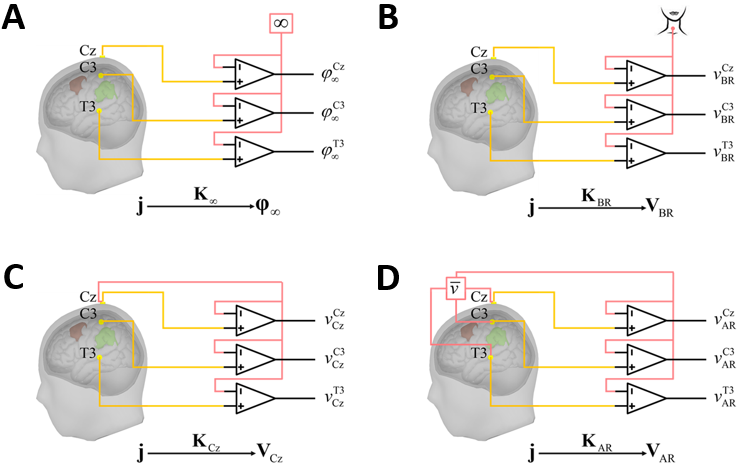
\includegraphics[width=15cm]{pic/Frontier/figure1.png}
	\caption{脑电参考问题图解}
	\label{3.1}
\end{figure}
为了精确定义这一问题,我们注意到这是由于脑电记录的固有本质是两个位点上的电势差。如图\ref{3.1}所示。理想情况下,人们希望用活跃电极只记录到部分脑组织产生的电活动信号,此时相对于具有零活动的中立参考电极。有人可能认为,参考电极应该放在无穷远,此时记录到的电位记为 $\mathbf{\phi}_{\infty}$。然而,这在实际中并不可行,因为这种无穷远放置好似一种天线,引入不必要的环境噪声。一些研究人员因而实验体表的参考电极以至于脑电差分放大器能够通过高的共模抑制比消除环境噪声。然而,因为体表上并无中立或者不活动的位点,这些提议也是不够的。一种物理上中立的参考似乎不望不可及。

然而,参考的不中立性具有到接下来一系列处理步骤的影响直到最终的处理结果。面对物理参考的不可能,注意力转移到虚拟中立参考估计量的构造,也即是$\mathbf{\phi}_{\infty}$的虚拟估计量。

一种广泛使用的虚拟估计量是如图\ref{3.1}D所示的平均参考(AR),其基于一下逻辑:
1)在内部只有电流源的球体内,球面上的电势积分为0\citing{goldman_clinical_1950,offner_eeg_1950}; 2)头表可以近似为球面; 3)中立参考可能通过加权或平均所有电极上的活动得到。这种重参考即是从所有通道信号中减去这种平均信号。
不幸地是,最近的研究\citing{yao_is_2017} 已经动摇了平均参考的理论基础: 真实头表面的电位积分不是零。
\begin{figure}[!ht]
	\centering
	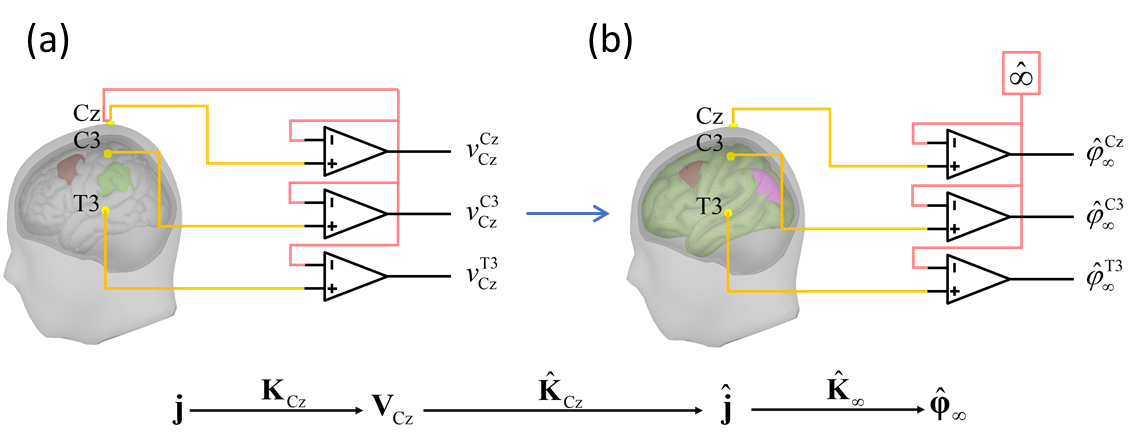
\includegraphics[width=15cm]{pic/Frontier/figure2.png}
	\caption{REST参考变换图解}
	\label{3.2}
\end{figure}
一种更加基于生物物理学的 $\mathbf{\phi}_{\infty}$ 虚拟估计量可以通过如图\ref{3.1}2所示的参考电极标准技术(REST)得到\citing{yao_method_2001}。REST采用一种头模型和等效源模型賴定位源活动,然后投射源活动到电极上,此时虚拟参考到无穷远。REST的早期工作是基于一种简单的球面头模型。 不久,脑电功率谱能量地形图\citing{yao_d_comparative_2005}和ERP峰值和潜伏期\citing{li_new_2007}的确高度依赖于参考的选择。 在进一步的研究中,\citing{tian_why_2013}研究发现 使用REST的头表SPM(统计参数成像)对听觉视觉刺激诱发电位研究比使用AR提供了更接近于通过LORETA的源定位结果。关于REST的令人鼓舞的结果通过一些仿真研究得到增强。采用球模型仿真,
\citing{marzetti_l_use_2007,qin_comparative_2010} 发现REST比AR得到更好的脑电谱和相干估计。 一些文章意料之中研究发现 REST采用真是头模型在仿真头表地形图重建 \citing{liu_q_estimating_2015},功能链接\citing{chella_impact_2016} 
和双谱分析 \citing{chella_f_non-linear_2017} 上都得到更好的结果。

\section{统一的参考估计量}
\subsection{广义脑电参考模型}
脑电总是基于一种时变的参考记录得到。 这常常被建模为从每个瞬时从所有电极上减去一个常数。大多数情况下,我们可以认为有两个不同的参考常数,一个相对于头表脑电信号,另一个相对于传感器电极噪声,如果噪声和大脑信号产生来自于不同的源。 这时,在线记录到的瞬时脑电信号可以用公式表示为:
\begin{equation}\label{eq3.1}
\mathbf{v}=\mathbf{\phi}-\mathbf{1}*\rho+\mathbf{\epsilon}-\mathbf{1}*\zeta
\end{equation}
这里,$\mathbf{\phi}$是采用中立参考的$N_{e}$通道干净脑电信号,也即是上面提到的$\mathbf{\phi}_{\infty}$,其分布是$N(\mathbf{0},\Sigma_{\mathbf{\phi}\mathbf{\phi}})$; $\mathbf{\epsilon}$ 是传感器电极噪声,其分布为$N(\mathbf{0},\sigma^{2}\mathbf{I}_{N_{e}})$。$\rho$和$\zeta$分别是脑电信号$\mathbf{\phi}$和$\mathbf{\epsilon}$的参考常量。$\rho$假设来自于大脑源活动,但$\zeta$可能来自大脑源、非大脑源或者二者的混合活动。由于这些常数的不确定性,$\mathbf{v}$的参考是一个未知变量。 注意到$\mathbf{\phi}$和$\mathbf{\epsilon}$的其他统计分布也适用于该相同的架构。参考起作用的过程起到了对脑电数据线性变化的作用,正式意义上,是对脑电数据矩阵左乘参考变换矩阵。因此,假设参考变换矩阵为$\mathbf{H=I-1f^T}$\citing{hu_how_2018},那么参考变化可以写作
\begin{equation*}
\mathbf{v}_{r}=\mathbf{Hv}=\mathbf{H(\phi+\epsilon)}-(\mathbf{I-1f^T})\times\mathbf{1}\times(\rho+\zeta)
\end{equation*}
注意到,等式$\mathbf{f^T1}=1$对所有的单点参考均成立,这些单点参考包括单点记录参考(例如Cz,Fz,Oz等),连接耳和平均参考。

因此,广义的脑电参考模型为
\begin{equation}\label{eq3.2}
\mathbf{v}_{r}=\mathbf{H\phi+e},\,\mathbf{e=H\epsilon}
\end{equation}
这里$r$指的是某一种参考。注意到$\mathbf{H}$是一个秩为$N_{e}-1$的矩阵。 因此,对$\mathbf{\phi}$的估计转换为一种欠定的广义线性逆问题。 通过最大后验估计\citing{p_murphy_machine_1991},或者最大惩罚似然估计\citing{eggermont_nonparametric_2009},我们得到如下目标函数:
\begin{equation}\label{eq3.3}
l=\mathbf{(v_{r}-H\phi)^{T}\Sigma_{ee}^{+}(v_{r}-H\phi)+\phi^{T}\Sigma_{\phi\phi}^{+}\phi}
\end{equation}
对\eqref{eq3.3}求对$\mathbf{\phi}$的偏导数得到
\begin{equation}
\hat{\mathbf{\phi}}=\mathbf{(H^T\Sigma_{ee}^{+}H+\Sigma_{\phi\phi}^{+})^{+}H^{T}\Sigma_{ee}^{+}V_{r}}
\end{equation}
根据矩阵逆变换引理\citing{hager_updating_1989,tarantola_inverse_2005},$\hat{\mathbf{\phi}}$可以重新表达为
\begin{equation}\label{eq3.4}
\hat{\mathbf{\phi}}=\mathbf{\Sigma_{\phi\phi}H^{T}(H\Sigma_{\phi\phi}H^{T}+\Sigma_{ee})^{+}v}_{r}
\end{equation}
此表达式就是重建无穷远参考脑电电位时统一的贝叶斯估计量。

为了推导出\eqref{eq3.4}的显式表达式,在假设分布$\mathbf{\Sigma_{ee}}=\sigma^{2}\mathbf{HH^T}$的基础上,$\mathbf{\Sigma_{\phi\phi}}$服从如下的两种形式。
\subsection{不相关的协方差先验}
\begin{equation}\label{eq3.5}
\mathbf{\Sigma_{\phi\phi}}=\alpha^{2}\mathbf{I_{N_{e}}}
\end{equation}
这意味着脑电信号$\mathbf{\phi}$具有所有电极间空间意义上的独立先验,$\alpha^{2}$是所有电极上脑电信号的方差的平均值。

将\eqref{eq3.5},$\mathbf{v}_{r}=\mathbf{Hv}$和$\Sigma_{ee}=\sigma^{2}\mathbf{HH^{T}}$代入\eqref{eq3.4}得到
\begin{equation}\label{eq3.6}
\hat{\phi}=\mathbf{H^{+}Hv}/(1+\sigma^{2}/{\alpha^{2}})
\end{equation}
在附录中,我们证明了$\mathbf{H^+H}=\mathbf{I}_{N_e}-11^T/N_e$就是平均参考转换矩阵。定义电极噪声相对于头表脑电信号比例为$nsr_1=\sigma^2/\alpha^2$,同时定义$\mathbf{H}_{ar}=\mathbf{I}_{N_e}-\mathbf{11^T}/{N_e}$,\eqref{eq3.6}可以写为
\begin{equation}\label{eq3.7}
\hat{\mathbf{\phi}}=\mathbf{H}_{ar}\mathbf{v}/(1+nsr_1)
\end{equation}
这就成为正则化的平均参考(rAR)。显然,传统的AR是rAR当$nsr_1=0$时的特例。
\subsection{相关的协方差先验}
\begin{equation}\label{eq3.8}
\Sigma_{\mathbf{\phi\phi}}=\mathbf{K}_{\infty}\Sigma_{\mathbf{jj}}\mathbf{K}_{\infty}^T
\end{equation}
该等式建立了所有电极上脑电电位的相关性,这种相关性是由于神经源活动容积传导效应,即我们假设$\mathbf{\phi}=\mathbf{K}_{\infty}\mathbf{j}$。$\mathbf{K}_\infty$指的是无穷远参考下得到的传递矩阵;$\mathbf{j}$神经源活动的主要电流密度,具有分布$\mathbf{j}\sim{N(\mathbf{0},\beta^2\mathbf{I}_{N_s})}$;$\beta^{2}$是多变量高斯信号$\mathbf{j}$的方差。

我们定义$\mathbf{K}_{r}=\mathbf{HK}_{\infty}$,并代\eqref{eq3.8}入\eqref{eq3.4}得到
\begin{equation}\label{eq3.9}
\hat{\mathbf{\phi}}=\mathbf{K}_{\infty}\Sigma_{\mathbf{jj}}\mathbf{K}_{r}^{T}\mathbf{(\mathbf{K}_{r}\Sigma_{\mathbf{jj}}\mathbf{K}_{r}^{T}+\Sigma_{ee})^{+}v}_{r}
\end{equation}
该表达式就是重建无穷远参考的脑电电位的估计量,记为正则化的参考点击标准化技术(rREST)。这个参考变换过程可以理解为两个步骤:
步骤一:$\hat{\mathbf{j}}=\Sigma_{\mathbf{jj}}\mathbf{K}_{r}^{T}\mathbf{(\mathbf{K}_{r}\Sigma_{\mathbf{jj}}\mathbf{K}_{r}^{T}+\Sigma_{ee})^{+}v}_{r}$
步骤二:$\hat{\mathbf{\phi}}=\mathbf{K}_{\infty}\mathbf{j}$
其中,步骤一采用传递矩阵$\mathbf{K}_{r}$解决了逆问题,该传递矩阵含有和脑电信号$\mathbf{v}_{r}$相同的参考,步骤二进行正演计算来重建理论的中立参考的脑点电位。 步骤一中的$\hat{\mathbf{j}}$ 是同时解决线性逆问题和参考问题的标准形式。

我们定义电极噪声对大脑神经源活动信号比为$nsr_{2}=\sigma^{2}/\beta^{2}$,代入$\sigma_{\mathbf{jj}}=\beta^{2}\mathbf{I}_{N_{s}}$和$\sigma_{\mathbf{ee}}=\sigma^{2}\mathbf{HH^{T}}$到\eqref{eq3.9},我们得到:
\begin{equation}\label{eq3.10}
\hat{\mathbf{\phi}}=\mathbf{K}_{\infty}\mathbf{K}_{r}^{T}(\mathbf{K}_{r}\mathbf{K}_{r}^{T}+nsr_{2}\mathbf{HH^{T}})^{+}\mathbf{v}_{r}
\end{equation}
这就是通过引入等对角线结构$\sigma_{\mathbf{jj}}$解决逆问题来重建无穷远参考的脑电电位的解。显然,REST\citing{yao_method_2001}$\hat{\mathbf{\phi}}=\mathbf{K}_{\infty}\mathbf{K}_{r}^{+}\mathbf{v}_{r}$是如\eqref{eq3.10}中rREST当$nsr_{2}=0$的特例。为了清晰可见,我们归纳总结广义参考模型和统一的参考估计量如表一所示。

\section{参考比较}
表一所示,如果电极噪声为零或者不采用正则化技术,AR和REST就分别是rAR和rREST的特例。在本小节中,转换广义参考模型到标准的脊回归形式后,我们采用统计模型准则评价参考估计量。
\subsection{标准回归形式}
参考估计的目标函数\eqref{eq3.3}等价于广义脊回归形式\citing{chung_optimal_2014}:
\begin{equation}\label{eq3.11}
\hat{\mathbf{\phi}}(\lambda)=\mathbf{\phi}\underbrace{argmin}{\lVert\mathbf{V}_{r}-\mathbf{H\phi}\rVert_{M}^{2}+\lambda\lVert\mathbf{L\phi}\rVert_2^2}
\end{equation}
这里$\lambda>=0$是正则化参数,$\mathbf{L}$是正则化矩阵。方便起见,我们也称$\lambda$和$\mathbf{L}$ 的正则化作用分别为参数正则化和结构正则化。
脊回归是Tikhonov正则化的统计学名字\citing{hoerl_ridge_1970}。脊回归的广义与标准形式的差别在于是否正则化矩阵$\mathbf{L}$是单位矩阵,是否失匹配项是欧式模\citing{chung_optimal_2014}。 由此,我们重定义$\mathbf{\phi^\prime=L\phi}$ 以至于正则化矩阵成为单位阵,同时$\mathbf{e^\prime=D^{T}U^{T}e}$(分解$\mathbf{HH^{T}=USU^{T}}$和$\mathbf{S}^{+}=\mathbf{DD^{T}}$)以转换失匹配项从Mahalanobis模为欧式模。最终,标准的脊回归形式化为
\begin{equation}\label{eq3.12}
\hat{\mathbf{\phi}}^\prime(\lambda)=\mathbf{\phi}^\prime\underbrace{argmin}{\Vert{\mathbf{V}_{r}^\prime-\mathbf{H^\prime\phi^\prime}}2^2+\lambda\Vert{\mathbf{\phi}^\prime}_2^2}
\end{equation}
这里,$\mathbf{V}^\prime_r=\mathbf{D^{T}U^{T}v}_{r}$,$\mathbf{H}^\prime=\mathbf{D^{T}U^{T}HL^{+}}$。然后,$\mathbf{\phi}^\prime$关于$\mathbf{V}^\prime_r$的后验均值是
\begin{equation}\label{eq3.13}
\mathbf{\phi}^\prime=(\mathbf{H^{\prime^T}}\mathbf{H}^\prime+\lambda\mathbf{I}_{N_e})^+\mathbf{H^{\prime^T}}\mathbf{v}^\prime_r
\end{equation}
那么,关于$\mathbf{\phi}$的估计就是$
\mathbf{\phi}^\prime=\mathbf{L}^\prime(\mathbf{H}^{\prime^T}\mathbf{H}^\prime+\lambda\mathbf{I}_{N_e})^+\mathbf{H}^{\prime^T}\mathbf{v}^\prime_r$,该等式等价于\eqref{eq3.10}。
\subsection{模型选择准则}
因为脊回归形式是一种线性估计量($\hat{\mathbf{v}^\prime_r}={\mathbf{Pv}^\prime_r}$),$\mathbf{P}=(\mathbf{H^{\prime^T}}\mathbf{H}^\prime+\lambda\mathbf{I}_{N_{e}})^{+}\mathbf{H^{\prime^T}}$作为投影(hat)矩阵。平方和误差(residual sum square error (RSS))定义为
\begin{equation}
RSS=\sum_{t=1}^{N_{t}}\lVert\mathbf{v}^\prime_{rt}-\mathbf{H}^\prime\mathbf{\phi}^\prime_t\rVert_2^2
\end{equation}
这里$\mathbf{v}^\prime_{rt}$和$\mathbf{\phi}^\prime_{t}$指的是$\mathbf{v}^\prime_r$和$\mathbf{\phi}^\prime$在$t^{th}(t=1,...,N_t)$个时间点,$N_t$是整个脑电记录的时间点的个数。

在\eqref{eq3.12}的标注脊回归形式下,我们探究进行模型选择的三个信息准则:广义交叉验证(GCV)\citing{chung_optimal_2014}, Akaike信息准则(AIC),和Bayesian信息准则(BIC)\citing{konishi_information_2008} 来比较图表一中的参考估计量。为此,我们定义自由度
\begin{equation}
DF=tr(\mathbf{P})=\sum_{i=1}^{N_{e}}\dfrac{s_i}{s_i+\lambda}
\end{equation}
这里$s_i$是$\mathbf{H}^{\prime^T}\mathbf{H}^\prime$的特征值。因为脑电参考相当于单个时刻点所有电极上加上或减去一个时变常数,这种瞬时效应造成了时域上的动力学失真。为探究参考的差异,我们近似地推广模型选择准则从单个时刻点到全局记录。预定义$N_{et}=N_eN_t$,GCV,AIC和BIC可以表示为
\begin{equation}\label{eq3.14}
GCV(\lambda)=RSS/(N_{et}-DF)^2
\end{equation}
\begin{equation}\label{eq3.15}
AIC(\lambda)=N_{et}log(RSS/{N_{et}})+N_t\cdot{2}\cdot{DF}
\end{equation}
\begin{equation}\label{eq3.16}
BIC(\lambda)=N_{et}log(RSS/{N_{et}})+N_t\cdot{DF}\cdot{log(N_{et})}
\end{equation}
注意到单个时刻点下GCV,AIC,和 BIC 分别是\eqref{eq3.14},\eqref{eq3.15},\eqref{eq3.16}在$N_t=1$的特例。
\subsection{正则化参数}
正则化参数$\lambda$平衡了对于数据模型拟合的效果与无穷远参考下脑电信号的先验限制。 
人们可能尝试通过迭代交互式地层级贝叶斯超参数\citing{mackay_bayesian_1992,trujillo-barreto_bayesian_2004}。 然而这可能对rREST有效但对rAR却得到比较差的效果因为rAR中的噪声项会因独立相同的协方差先验吸收进\eqref{eq3.6}中的干净脑电信号。 即,AR的目标函数是非凸的,无法收敛到全局或者局部最优点。因此,我们采用搜索策略探究DF, GCV, AIC 和
BIC 如何随着$\lambda$的值而变化\citing{phillips_empirical_2005}。 方法是画出$DF$随着$\lambda$以及 GCV, AIC和BIC随着$DF$变化的曲线。\eqref{eq3.7}和\eqref{eq3.10}的理论结果表明最优的$\lambda$对于rAR来说接近$nsr_1$,对于rREST来说接近$nsr_2$。 因为容积传导效应相当于一个低通时空滤波器,这就会导致$nsr_2 ≪ nsr_1$
\citing{srinivasan_r_spatial_1998,stinstra_volume_1998,srinivasan_methods_1999,nunez_electric_2006}。假设信噪比的区间对于rREST是[35, 10] dB, 对于rAR来说是[30, −10] dB,我们用采样算法随机生成1000个$\lambda$对于rREST来说从$10^{-3.5}$到0.1,对于rAR老说从$10^{-3}$到0.1。

在仿真中,我们可以设定基准——最优的正则化参数比较参考估计量,即该参数下可以得到相对于基准电位的最小相对误差。另外,模型选择准则(GCV,
AIC,和BIC)的对选择正则化参数效果可以得到比较。实际脑电数据中,因为基准脑电数据是未知的,所以找到一个合适的$\lambda$会更加困难。 当模型选择准则达到全局或者局部最优时的参数$\lambda$视为真实脑电数据分析中该模型选择准则的最优$\lambda$值。

\cite{yao_method_2001}中建议在使用REST时避免采用正则化参数以免丢失高频信息。 另外,\cite{zhai_y_and_yao_d_study_2004}提出在使用REST时候可以采用截断奇异值的分解方法以抑制电极噪声。因此,我们经验地选择REST中推荐的截断参数0.05,但是在rREST中仍然采用模型选择准则。
\section{正则化矩阵}
正则化矩阵$\mathbf{L}$的选择依赖于无穷远电位的先验协方差结构。表一列出了$\mathbf{\phi}$的先验协方差结构对于AR和rAR来说$\Sigma_{\mathbf{\phi\phi}}=\alpha^{2}\mathbf{I}_{N_e}$,$\Sigma_{\mathbf{\phi\phi}}=\mathbf{K}_{\infty}\Sigma_{\mathbf{jj}}\mathbf{K}_{\infty}^T$对于REST和rREST。 因此,$\mathbf{L}$的选择是:\\
对于AR和rAR,$\mathbf{L}_ar=\mathbf{I}_{N_e}$\\
对于REST和rREST,
\begin{equation}\label{eq3.17}
\mathbf{L}_rt=[(\mathbf{K}_{\infty}\mathbf{K}_{\infty})^{T+}]^{1/2}
\end{equation}

$\mathbf{K}_{\infty}$的一些例子在下一节中详细讨论列出。 $\mathbf{L}_{rt}$中具有的生物物理学信息的正则化程度从对容积传导模型的不太切合实际的近似到更加切合实际的增加。
\subsection{容积传导模型}
对于rREST,我们研究可能涉及到的容积传导模型匹配问题,就是,在哪种程度上,rREST的传递矩阵可能偏离实际真实的传递矩阵,无论仿真脑电还是真实的脑电都是从传递矩阵得到。这里,我们研究几种不同类型的传递矩阵:熟知的球形传递矩阵(SLF)是一种频繁采用的标准传递矩阵,最精确的容积传导模型是个体被试匹配了机构MRI数据的个体传递矩阵(ILF),还有被试群体平均的传递矩阵(ALF)作为个体被试传递矩阵的替代品。我们也研究了个体被试稀疏源的传递矩阵(sILF),仿真中没有未激活的源被关闭。 我们用后缀来区别不同类型的传递矩阵。
\subsubsection{球形传递矩阵 (SLF)}
$\mathbf{K}_{\infty}^{s}$是基于三层同心球面模型生成。三层分别是大脑皮层、颅骨、头表,相对传导率分别为1,0.0125和1,三层的球面相对半径对头皮和颅骨内外表面分别是1.0,0.92和0.87。 源空间由2600个均匀垂直于皮层表面半径为0.86的离散偶极子和400个均匀垂直于水平半径为$z=-0.076$断面偶极子组成。这里,传导率、半径和坐标的值都不是实际的测量值而是层与层之间传导率和半径的相对比例,以及单位球面空间中的相对坐标值\citing{yao_method_2001,hu_how_2018}。
\subsubsection{个体传递矩阵(ILF)}
$\mathbf{K}_{\infty}^i$通过归一化定义为
\begin{equation*}
\mathbf{K}_{\infty}^i=\mathbf{K}_{\infty}^{iraw}/{[\Tr(\mathbf{K}_{\infty}^i\mathbf{K}_{\infty}^iT)]^{1/{2}}}
\end{equation*}
这里$\mathbf{K}_{\infty}^{iraw}$是与古巴人类脑影像计划
\citing{uludag_latin_2009,valdes-hernandez_white_2010,hernandez-gonzalez_multimodal_2011,bosch-bayard_3d_2012}
中接受脑电记录的$i^{th}=1,...,N_b$被试相匹配的原始个体传递矩阵。 
原始的个体传递矩阵时基于结构磁共振数据用CIVET大脑皮层表面分割流程\citing{ad-dabbagh_civet_2006}和有限元方法估计得到的。 大脑皮层表面由6003个顶点和11998*3个面组成。 总共,6003各偶极子源分布在各个顶点上,分别垂直于皮层表面激活。对不同被试个体的传递矩阵归一化使得被试间的相互比较。

\subsubsection{平均传递矩阵(ALF)}
$\mathbf{K}_{\infty}^a$是$N_b$个被试的所有归一化的个体传递矩阵的平均,用等式表示为:
\begin{equation*}
\mathbf{K}_{\infty}^a=\frac{1}{N_b}\sum_{i=1}^{N_b}\mathbf{K}_{\infty}^i
\end{equation*}

\subsubsection{稀疏化个体传递矩阵(sILF)}
$\mathbf{K}_{\infty}^{si}$,由于稀疏的程度只有仿真中已知所以其只在仿真中使用,首先转换为个体传递矩阵(ILF),然后通过如下计算获得
\begin{equation*}
\mathbf{K}_{\infty}^{si}=[\mathbf{K}_{\infty}^{iraw}\circ\mathbf{W}_i]/{[\Tr(\mathbf{K}_{\infty}^{iraw}\circ\mathbf{W}_i\mathbf{W}_i^T\circ{\mathbf{K}_{\infty}^{iraw}}^T)]^{1/2}}
\end{equation*}
这里$\circ$指的是矩阵元素元素之间的乘操作,即Hadamard积; $\mathbf{W}_i$是一个和$\mathbf{K}_{\infty}$具有相同行和列数由二值权重组成的矩阵; 在未激活的神经源对应列的元素权威零,其它列全为1。 仿真中,两个源块的位置信息被引入到使用rREST对无穷远参考下脑电电位的空间协方差中。 而不是采用$\ell_0$或者$\ell_1$来稀疏化大脑神经源信号$\mathbf{j}$,我们直接设个体传递矩阵中对应于非激活神经源的元素为零以间接地约束大脑神经源信号。

\section{结果}
\subsection{仿真}
\subsubsection{脑电生成}
仿真思路是基于如下的正演计算公式:
\begin{equation}\label{eq3.18}
\begin{split}
\mathbf{v}_r=\mathbf{H\phi}+\mathbf{H\epsilon},\mathbf{\phi}=\mathbf{K}_{\infty}^{iraw}\mathbf{j}\\
SNR=10log_{10}(\alpha^2/\sigma^2)
\end{split}
\end{equation}
这里$\mathbf{v}_r$是基于单极参考仿真出的脑电电位;不是一般性,线性结合向量$\mathbf{f}=[0,...,0,1]^T$仅最后一个元素为1其他均为零;如图\ref{3.3}所示,在神经源$\mathbf{j}$中有两个源块包含的150个偶极子被激活,满足四阶双变量自回归模型;信噪比SNR是头表脑电信号与传感器电极噪声方差之比,以分贝dB为单位。
\begin{figure}[!ht]
	\centering
	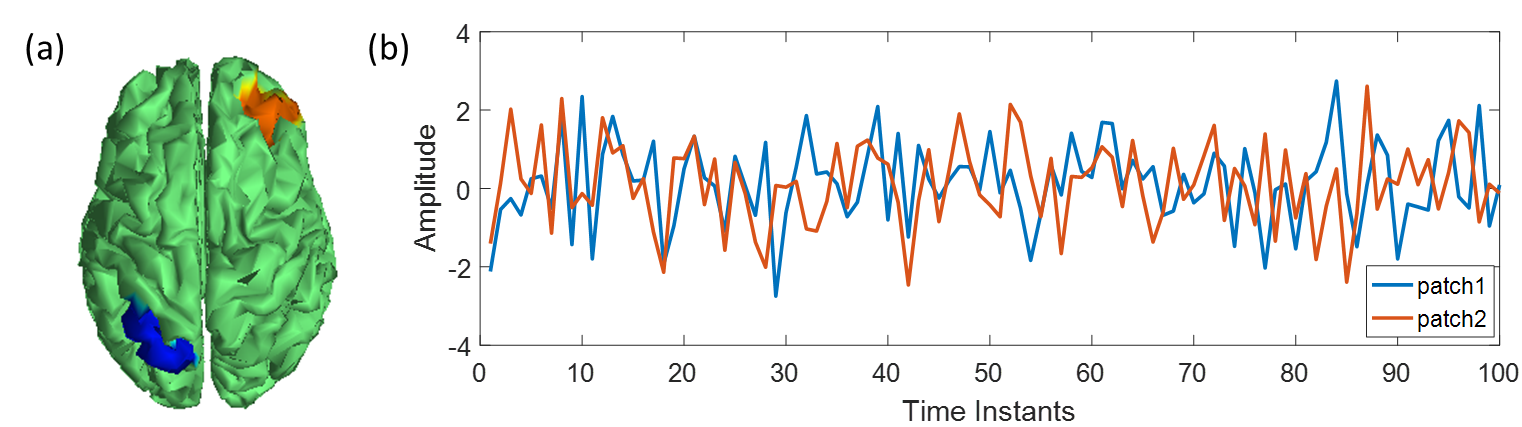
\includegraphics[width=15cm]{pic/Frontier/figure3.png}
	\caption{仿真脑电电位所用的神经源活动}
	\label{3.3}
\end{figure}
使用古巴人类脑影像数据库中的89个被试的个体传递矩阵$\mathbf{K}_{\infty}^{iraw}$,仿真的每组脑电数据是89被试$\ast$58通道$\ast$5120时刻点。 总共,我们仿真生成了数据集A:4 组数据,信噪比SNR组内相同组间不同, 数据集B:一组数据,SNR对所有的被试个体都不同。 仿真给出了基于中立无穷远参考的脑电电位的基标准,使得就相对脑电电位误差而言直观地比较参考的效果成为可能。 对每个被试的脑电数据来说,脑电电位的相对误差定义为
\begin{equation}\label{eq3.19}
RE=\lVert\hat{\mathbf{\phi}}-\mathbf{\phi}\rVert^2_F/{\lVert\mathbf{\phi}\rVert^2_F}
\end{equation}
这里$\mathbf{\phi}$值得是仿真出的脑电电位基标准,$\hat{\mathbf{\phi}}$是用参考估计量估计出的脑电电位。

\subsubsection{参考估计量的相对误差}
仿真数据集A中具有4组数据,其SNR值分别设为20,8, 4,2分贝以此用来计算参考前后相对误差。 图\ref{3.4}A–D显示了REST和rREST参考估计量的相对误差,分别具有四种传递矩阵的情况 (SLF, ILF, ALF, and sILF) 。 黑绿红蓝的柱状图分别表示了AR,rAR,REST和rREST的相对误差。 显然从图\ref{3.4}A–D的柱状图可以看出,正则化参考(rAR, rREST)的相对误差总小于没有正则化的参考(AR,REST)的相对误差。 非配对型的t检验用以检查非正则化参考(AR,REST)与正则化参考(rAR,rREST)之间的差异。图\ref{3.4}E列出了AR与rAR之间的统计显著性水平(即p值),以及使用各种不同传递矩阵时REST与rREST之间的显著性水平。 除了AR与rAR在SNR=20分贝时的情况, p值都达到非常小的值(<1e-7)。使用正则化,从REST到rREST相对误差的下降比着从AR到rAR的下降更加明显。 尤其是,使用稀疏化的个体传递矩阵进行正则化比着球面传递矩阵、个体传递矩阵、被试平均的传递矩阵更加有效得多。 这是意料之中的结果,因为神经源活动的稀疏先验信息引入到了协方差结构中。 相比之下,使用最简单的容积传导模型即球面传递矩阵,当SNR=20或者8分贝时,rREST的相对误差似乎甚至比AR的大,在所有的参考REST体现了最差的效果。 把稀疏化个体传递矩阵的相对误差和球面传递矩阵时rREST的相对误差与使用球面传递矩阵REST的相对误差,我们发现使用准确协方差的结构正则化似乎比选择最优的$\lambda$进行参数正则化更加有效, 最优的$\lambda$是在所有测试的$\lambda$中产生了最小的相对误差的那个。 使用稀疏化个体传递矩阵的rREST的相对误差是所有其他参考相对误差中最小的情况。 这意味着结构正则化结合参数正则化会达到最优的效果。 另外,引入更高的传感器电极噪声使得SNR从20分贝降低到2分贝,rAR的相对误差相应地从少于$15\%$增加到高于$60\%$,相比之下,除去球面传递矩阵的情况rREST的相对误差从$4.1\%$增加到$40\%$。
\begin{figure}[!ht]
	\centering
	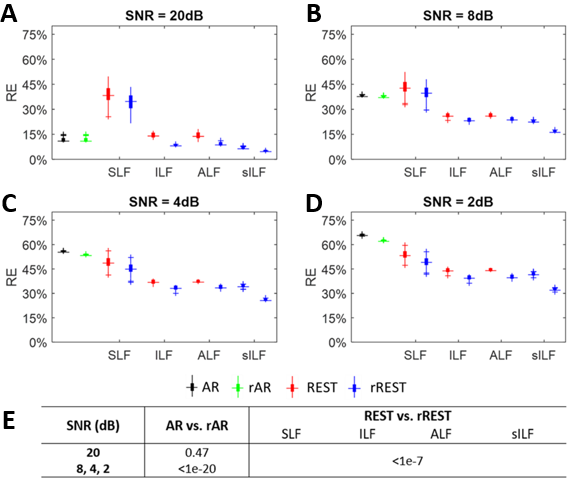
\includegraphics[width=15cm]{pic/Frontier/figure4.png}
	\caption{参考估计量的相对误差}
	\label{3.4}
\end{figure}
这些结果表明:(1) 除了AR和rAR在SNR等于20分贝的情况,AR,rAR和使用粗略地近似实际容积传导模型的球面传递矩阵的REST和rREST可能无法重建无穷远参考下的脑电信号,这可以根据此时十分大的相对误差看出; (2) REST和rREST的效果依赖于容积传导模型; (3) 使用更严格的正则化,rREST可以获得更好的效果; (4) 对于REST和rREST来说,使用被试群体平均的传递矩阵的相对误差似乎达到了和使用被试个体传递矩阵几乎一致的误差; (5) rAR可能没有去噪的效果。 总之,当SNR非常高(大于等于20分贝)时,AR和rAR可能作为一种rREST的替代选择,当然具有准确容积传导模型时的rREST应当成为估计无穷远参考下脑电电位的首选。

\subsubsection{用仿真数据对参考估计量进行模型选择}
我们分析仿真数据集B来进行模型选择,在仿真数据集B中89个样本被设置为具有随机均匀分布在间隔[5 20]分贝的SNR值以模仿实际脑电记录中被试之间不同的SNR的情况。 汇总在图\ref{3.5}中的结果可以让我们通过模型选择准则选择最优的参考。 画出的DF (自由度),RSS(残差平方和), 以及模型选择准则(GCV,AIC,BIC) 是89个数据样本中逐一地在单个数据样本关于所有检测到的正则化参数$\lambda$的平均。
图\ref{3.5}A中的曲线显示了DF和GCV如何随着$\lambda$的变化而变化以及RSS如何随着DF的变化而变化。容易看出rREST的DF总是比rAR的DF更小一些。 这意味着rREST比rAR采用了更简单的模型来重建无穷远参考下的脑电信号但是利用了更加实际的先验信息来进行正则化。 rREST比rAR更低的RSS表明rREST重建得到的脑电信号相对于rAR重建得到的脑电信号更接近于仿真的基标准。 图\ref{3.5}B的曲线显示了模型选择准则(GCV, AIC, BIC) 如何随着DF变化而变化。 显然,rREST的模型选择准则总比rAR的更小。 模型选择准则普遍更低的值给出了rREST相对于rAR具有优势的证据。
\begin{figure}[!ht]
	\centering
	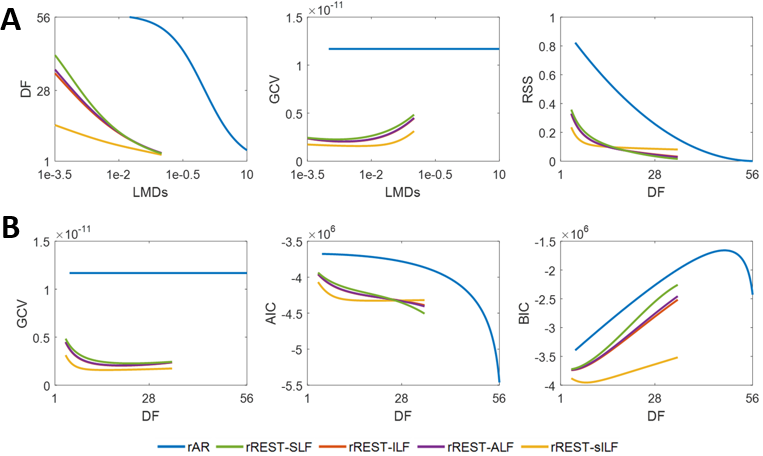
\includegraphics[width=15cm]{pic/Frontier/figure5.png}
	\caption{用仿真数据进行模型选择}
	\label{3.5}
\end{figure}

\subsubsection{正则化参数}
对于rREST,选择最优的正则化参数,即$\lambda$的值是至关重要的。 图\ref{3.6}显示了模型选择准则(GCV,AIC和BIC)选出的$\lambda$的值在多大程度上和基标准的正则化参数的接近程度,基标准的正则化参数是由基于仿真数据集B参考前后具有最小的相对误差的准则挑选出来的。 注意到通过基标准识别出的最优的$\lambda$和模型选择准则的计算是在个体被试数据水平并非被试群体水平,因为这是在个体水平上利用了关于所有测试的$\lambda$平均化的模型选择准则曲线。 把图\ref{3.6}B–D中的平均相对误差(mRE)和标准偏差和图\ref{3.6}A中的相比较,我们容易发现GCV是选择恰当的正则化参数最优的一个,
因为用GCV得到与基标准几乎一致的平均相对误差和标准偏差。 AIC不如GCV,这是因为除了rREST用稀疏化的个体传递矩阵时,正则化的参考(rAR, rREST)具有和普通的参考(AR, REST)相同或更大的平均相对误差和标准偏差; BIC是最不适合用于选择恰当的正则化参数,因为所有的正则化参考得到了比普通的参考(AR, REST)更大的平均相对误差和标准偏差。
\begin{figure}[!ht]
	\centering
	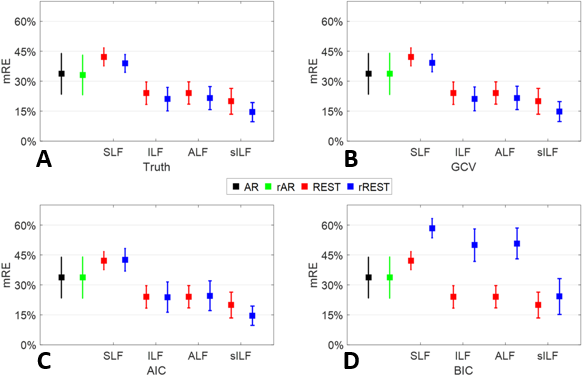
\includegraphics[width=15cm]{pic/Frontier/figure6.png}
	\caption{正则化参数选择}
	\label{3.6}
\end{figure}

\subsection{用真实数据对参考估计量进行模型选择}
我们用古巴人类脑成像数据库中的89个被试的脑电数据賴评价参考估计量。对被试进行脑电记录的实验经过公共健康部伦理道德委员会和古巴神经科学中心的批准,每个被试都签有实验知情同意书。 脑电采集共58个电极,10-10电极放置系统,采样率200Hz,记录时间每个被试2.5到5分钟。 对于每个被试,我们分别用被试个体的传递矩阵、稀疏化的个体传递矩阵、平均传递矩阵和球面传递矩阵进行REST变换,并且计算了GCV、AIC和BIC三种模型选择准则。 模型选择准则又在89个被试之间进行平均。 
\begin{figure}[!ht]
	\centering
	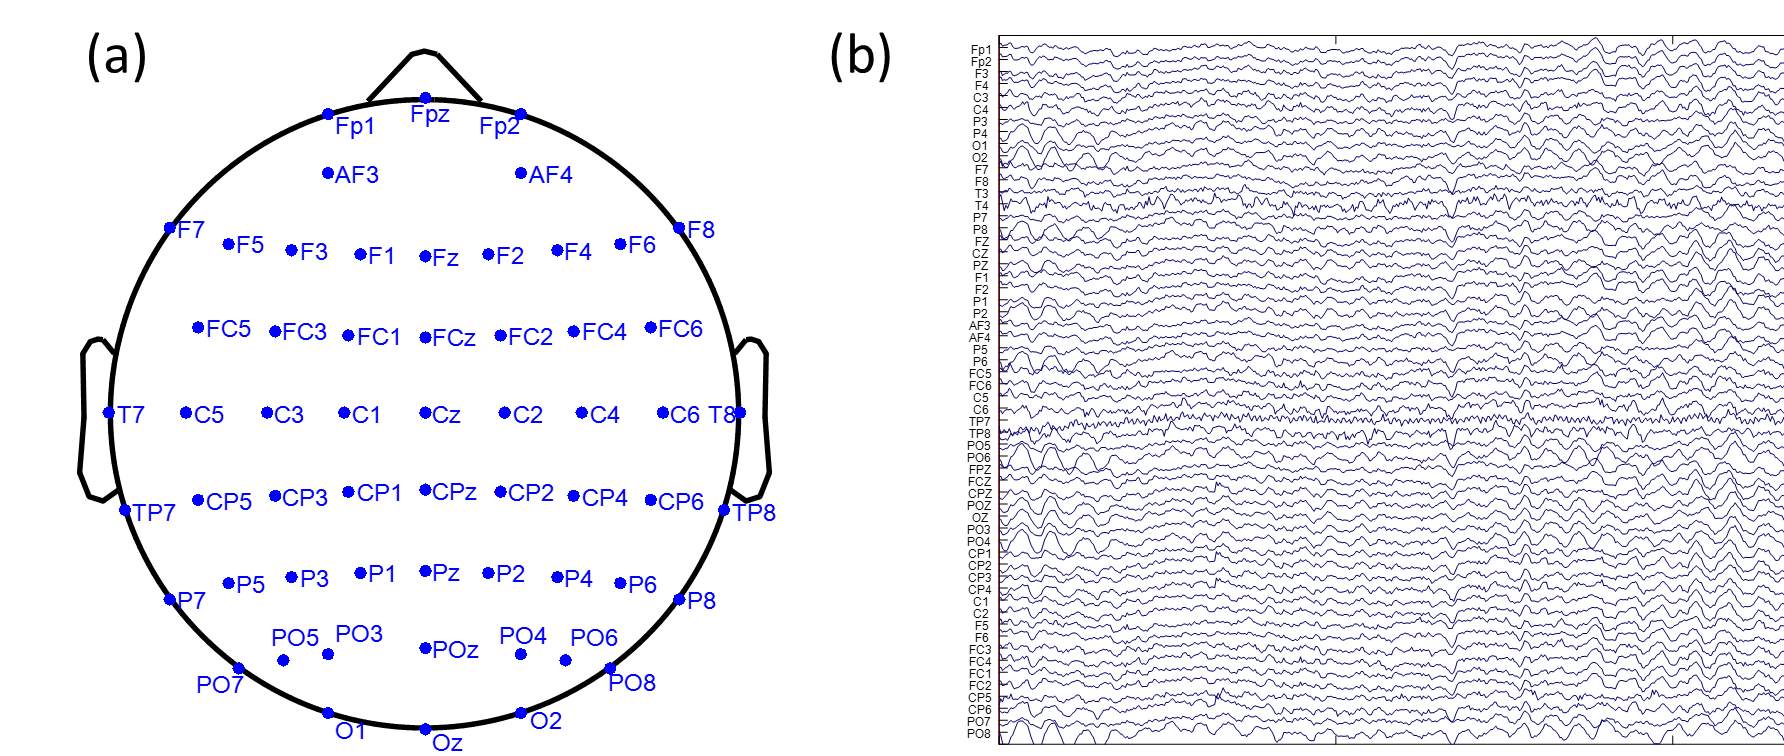
\includegraphics[width=15cm]{pic/Frontier/figure7.png}
	\caption{真实脑电数据示例}
	\label{3.7}
\end{figure}
为了验证rREST比rAR更好,一种与仿真中比较参考效果的相似分析运用在古巴人类脑成像数据库中的89个被试的实际的静息态脑电数据。 图\ref{3.8}中的结果显示了DF(自由度)和GCV(广义交叉验证)如何随着正则化参数$\lambda$的变化而变化以及RSS(参差平方和)和模型选择准则(GCV,AIC和BIC)如何随着DF的变化而变化。 图中画出的DF,RSS和模型选择准则是89个被试逐一分析后在被试之间进行平均的结果。 因为参考转换矩阵$\mathbf{H}$和正则化参数$\lambda$ (即LMD)的区间和仿真中的设置一致,图\ref{3.8}A中DF随着LMD变化的曲线就和图\ref{3.5}A中的完全一致。图\ref{3.8}B中更低的RSS和模型选择准则曲线说明用真实数据验证了仿真中的结果(1)rREST重建的脑电信号具有比rAR重建的信号更低的RSS;(2)除了在DF≈28时rREST和rAR具有几乎一样的BIC的情况,在其他情况下rREST比rAR都具有更小的GCV,AIC和BIC。 因为在图\ref{3.6}中,我们发现GCV是在仿真中选择恰当正则化参数$\lambda$的最优准则,我们建议当实际数据分析中基标准未知时采用GCV对每一个脑电记录选择$\lambda$的值。 图\ref{3.8}A中的中间的曲线说明GCV的值如何随着$\lambda$的值变化。 对于rREST,GCV在$\lambda=1e-2$或者DF=10附近达到全局最小值。 因此,我们推断在实验数据组分析中有可能通过最小的GCV找到最优的正则化参数,这可能为rREST使用中选择可能最优的$\lambda$提供了一个经验型例子。然而,如我们在图\ref{3.6}中所展示的,对每一个被试的脑电记录都用GCV选择正则化参数是更安全的。 相比之下,rAR的GCV曲线好像是一个常数曲线,这是因为rAR是非凸解就河南找到恰当的$\lambda$。 这些结果表明rREST相对于rAR的优势也在真实脑电数据中得到了验证。 另外,对于rREST,最优的正则化参数可在GCV曲线的全局最小值处选出。
\begin{figure}[!ht]
	\centering
	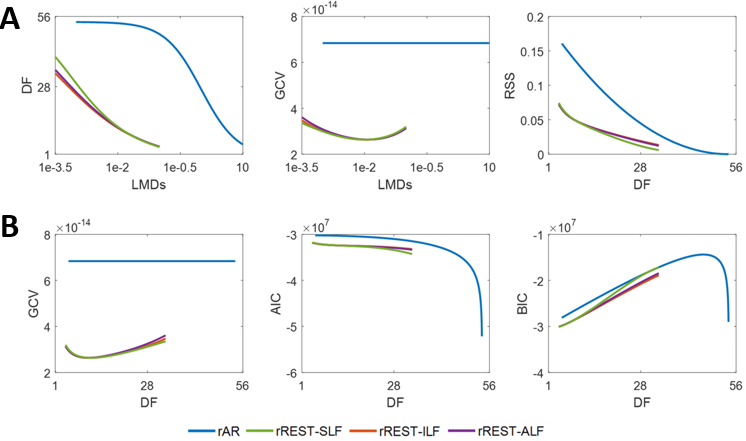
\includegraphics[width=15cm]{pic/Frontier/figure8.png}
	\caption{用真实脑电进行模型选择}
	\label{3.8}
\end{figure}

\section{讨论}
尽管REST已经提出了一段时间,它的理论基础还没有被深入研究过,特别需要的是从数理统计学的角度。REST提出之前,平均参考(AR)已经得到普遍采用,例如在微状态分析中\citing{khanna_microstates_2015},也作为逆问题中参考电极问题的最终解\citing{rd_pascual-marqui_review_1999,pascual-marqui_standardized_2002,pascual-marqui_discrete_2007,pascual-marqui_assessing_2011}。当前,AR和rEST是参考估计中的两个主要的具有竞争性地理论差异尚不明确的估计量 \citing{nunez_rest_2010}。 有许多关于二者的对比研究,然而,这些都没有提供明确的理论证据以支持其中之一的优越性
\citing{qin_comparative_2010,chella_impact_2016,chella_f_non-linear_2017,lei_x_and_liao_k_understanding_2017}。结束这种争论的必要被最近尧德中的理论结果加强,该结果证明了AR的主要物理学假设——头皮上脑电信号的平均作为对大脑参考信号的消除一般是错的\citing{yao_is_2017}。然而,仅仅从生物物理学的角度来解决参考问题可能是困难的。采用一种完全统计学模型用以最佳参考的先验验证也是必要的。

在本研究中,我们把无穷远参考下电位的估计和参考的选择看作一种线性逆问题,这种逆问题可以用熟知的贝叶斯技术来解决。令我们惊奇的是,AR和REST是具有两个不同的基于无穷远参考脑电电位空间协方差的先验分布的特例。通过显式地引入电极噪声到参考模型中,我们就把无穷远参考下电位估计和去噪结合起来了。基于最大后验估计的公式衍生出正则化的参考估计量,即rAR和rREST。最后,将参考视为线性逆问题,可以进行参考模型选择以及检测其他若干问题。对仿真和实际脑电数据,我们都发现 (1) 正则化对同时解决参考问题和去噪是很重要的。(2) 正则化的参考 (rAR/rREST) 比非正则化普通的参考具有更好的性能
(AR/REST)。(3) rREST优于rAR。 (4) 在应用rREST到真实脑电数据,广义交叉验证是一种有效的指标賴选择最佳的正则化参数。 以我们的观点,支持rREST的根本证据是89例真实脑电数据中rREST89具有更小的广义交叉验证指标。这是第一次对参考进行先验比较,并利用到了近似于贝叶斯模型证据的信息准则。

我们也证明了AR并非参考电极问题的最终解\citing{pascual-marqui_assessing_2011}, 只是统一的参考估计量中不相关先验和无噪声情况的一种特例。\cite{pascual-marqui_assessing_2011}中Pascual-Marqui et al 推导出了AR是利用了完全无噪声的假设,或者说在测量噪声的协方差矩阵是单位阵的条件下。在参考逆问题解之前,参考问题通过推导出的AR解决,这种AR被以为对参考过程食言了最佳的拟合。然而,在本章中,如果参考过程不仅存在于脑电信号也存在于测量噪声中,AR就无法推导出来。 因为逆问题不取决于参考电极变换,AR和单极参考可以用来转换传递矩阵,以及在解逆问题之前转换脑电记录具有和传递矩阵相同的参考。 这在公式\eqref{eq3.9}rREST的执行步骤一中体现出来。 

REST也因为合乎理论的基础引人注意\citing{yao_method_2001,kayser_j_and_tenke_c_e_search_2010,nunez_rest_2010}。 然而,普通REST的一些研究并非都比AR取得更好的效果\citing{yao_method_2001,hu_how_2018}。 尽管当神经源活动垂直于大脑皮层或者浅表层偶极子源活动,普通的REST比AR更加有效,但对于水平断面或者深层的偶极子并非如此。 尽管这些发现,我们认为是由于普通的REST的协方差结构来自于两个因素,球形容积传导体,等效分布的偶极子层的有效神经源 \citing{yao_equivalent_2003}, 即,径向方向分布于二维皮层薄片栅格上的源\citing{yao_method_2001}。 相反,我们在本章中检测了更多不同类型的真实容积传导模型。另外,仿真研究是基于多个皮层上的小块源。 我们的结果表明更加切合实际的容积传导模型和源空间并没有让参考估计量具有更好的性能,实际中,REST在大多数例子中具有比AR更好的效果。

我们强调源模型的多种可能性和广义逆问题这个概念。因为REST数据广义逆问题,多种源\citing{daunizeau_bayesian_2006}和一般的三维分布源分布在大脑容积体素的每一个栅格点上 \citing{michel_eeg_2004}均可以为REST所用\citing{yao_d_high-resolution_2000}。 我们发现广义逆不尽相同,接下来有趣的研究可能是探究如何不同的源模型程序能使用在REST的变种中。

容积传导模型匹配测试发现REST和rREST都是依赖于容积传导模型的,以及足够逼真的容积传导模型的重要性。这与\citing{hu_how_2018,liu_q_estimating_2015}的研究结果一致。\cite{liu_q_estimating_2015}发现一种实际的容积传导模型对于传统的REST是重要的。 \cite{hu_how_2018}发现传统的REST依赖于容积传导模型但是不十分精确或者轻微扰动的传递矩阵不会恶化REST的效果太多。这个仿真研究发现利用更好的估计容积传导模型和源会带给参考估计量来更好的效果。sILF 对于rREST的容积传导模型测试中得到最小的相对误差意义显然,是因为先验的sILF匹配了正演计算。仿真研究的主要论点在于唤起对rREST先验准确性的认识,尽可能切合实际越好。毋庸置疑的是, 只能实现更切合实际的近似。将来,考虑到一种准确先验的不确定性的可能有用的方法是利用贝叶斯模型平均\citing{trujillo-barreto_bayesian_2004}。 然而,估计个体被试的传递矩阵要求被试的结构磁共振数据,一般情况下在临床中不易得到,这种要求显得十分计算昂贵。然而,我们发现被试群体平均的传递矩阵实现了几乎和严格个体被试传递矩阵几乎相同的效果。 这验证了没有个体磁共振数据时近似头模型的想法可能比较有用 \citing{valdes-hernandez_approximate_2009}。 rREST的一个关键点是选择最优的正则化参数,这也是统计学习研究中密切研究的一点\citing{konishi_information_2008}。 我们的仿真和用真实脑电数据的验证结果表明广义交叉验证是一个简单又敏感有效的指标从而使得参数选择得到解决。实际中,我们推荐采用广义交叉验证准则賴选择单个被试脑电记录的正则化参数。

本章研究的主要贡献是:
1. 我们提出参考估计是一个统一的贝叶斯线性逆问题。
2. 这个架构显式地把电极测量噪声建模为脑电生成模型的一部分。
3. AR和REST是线性逆问题的特例,前者采用了空间独立的先验,后者采用者由于容积传导形成的空间相关的先验。
4. 正则化的参考估计量,rAR和rREST可以同时进行参考估计和去噪。
5. 我们采用了模型选择准则(GCV, AIC, BIC)不仅用于选择超参数还可以比较模型进行模型选择。 GCV似乎是最敏感有效的一个。
6. 被试群体平均的传递矩阵可以在实际中作为个体传递矩阵的代替品以构造接近最优的参考估计量。

同时,本章还进行了一些扩展研究:
• 抑制噪声可能与参考估计和去噪结合起来。例如,明显离群值信号可以通过鲁棒统计学的设计的似然函数消除\citing{huber_robust_1981}。
• 先验分布中可以考虑更多的生物物理知识以更有效地分离脑电信号和电极噪声。 特别是对应于不同稀疏结构源模型的协方差结构可以对比研究\citing{paz-linares_spatio_2017}。
• 我们仅仅研究了脑电协方差矩阵的空间先验。动力学先验知识也能容易地考虑进来。时域上自相关可以模拟为状态空间模型并通过卡尔曼滤波器估计得到\citing{galka_solution_2004}。 另外,对频域或者时频域进行模拟都是可能的。
• 这种统计学架构也能通过结合我们组之前研究结果拓展到事件诱发电位的信号处理研究中 \citing{carbonell_random_2004}。

\section{本章小结}
我们研究发现脑电参考问题可以统一为逆问题的一种,其可以通过贝叶斯技术解决。据我们所知,这是对脑电参考问题的一种创新方案,这允许我们:采用正则化方法估计无穷远参考下的电势,证明了无穷远参考和平均参考是统一贝叶斯估计量的特例只是二者区别于脑电电势的空间协方差先验,同时引入去噪进入参考估计程序中,采用了模型选择准则来选择最优的参考估计量。模型选择的结果归纳为:正则化的参考(无穷远或者平均)优于传统的无穷远或平均参考,其中正则化的无穷远参考无论在仿真研究还是真实数据验证上都体现了最优的性能;容积传导模型的选择是基于被试个体的传递矩阵或者被试群体平均的传递矩阵。
在本章中,我们采用贝叶斯最大后验估计,发现无穷远参考和平均参考属于统一的统计学架构,其区别在于先验的不同,采用基于容积传导的头表电极协方差先验和无噪声理想情况下得到的是无穷远参考,采用独立同分布的头表电极协方差在无噪声情况下得到的是平均参考,有噪声的情况下均视为正则化的参考电极标准化技术。这种技术称为rREST,作为无穷远参考的脑电电势的改进的估计量,有希望在临床实践中得以推广使用。